\section{Обзор предметной области}
\subsection{Постановка задачи моделирования видеотрафика
с переменной битовой скоростью}

Пусть есть некоторая видеопоследовательность ---
последовательность изображений в цифровом RAW-формате.
Данная последовательность подвергается сжатию с помощью
некоторого видеокодера, сконфигурированного с целью
сохранения качества видео при переменном размере кадра.

В данной работе в качестве
используется H.264~\cite{}, один из распространённых
кодеков видео. Кадровая частота, размер кадров (разрешение)
и цветовое разрешение известны.

С точки зрения моделирования видеотрафика, сжатый видеопоток
можно представить как последовательность из $N$ кадров
размера $s_i,~i=1\dots N$. Внутренняя структура сжатого
кадра не рассматривается. Кадры, тем не менее, разделены
на три типа в зависимости от использования и типе межкадрового
предсказания (англ. inter-frame prediction)~\cite{}.
В стандарте H.264~\cite{} предусмотрено разбиение каждого
кадра на прямоугольные области одинакового размера (макроблоки),
для каждой из которых индивидуально определяется тип и наличие
предсказания, но с ограничением, определяемым типом всего кадра:

\begin{itemize}
    \item I-кадры (также называются ``ключевыми'', англ. intra-frames).
        Содержат только макроблоки, сжатые независимо от макроблоков
        других кадров.
    \item P-кадры (``разностные'' кадры, англ. predicted frames).
        Могут содержать как макроблоки, сжатые независимо от других
        кадров, так и макроблоки, сжатие которых осуществлялось с
        опорой на другой предшествующий I- или P-кадр.
    \item B-кадры (``двунаправленные'' кадры, англ. bi-predicted frames).
        Могут содержать макроблоки следующих типов: предсказанные с опорой
        на другой I-, P-, B-кадры или с опорой на два кадра любого в
        общем случае типа, один из которых предшествует текущему,
        а другой следует за текущим кадром.
\end{itemize}

Как правило, в видеокодеках используется некоторая техника
разностной импульсно-кодовой модуляции (англ. differential
pulse-code modulation, DPCM)~\cite{}, предполагающая некоторую
процедуру предсказания текущего макроблока по множеству других.
Выбор макроблоков, на основе которых производить предсказание,
и является критерием типизации макроблоков и кадров.

Наличие ``опорных'' кадров позволяет существенно ускорить
время получения произвольного кадра в потоке и ``быстрой
перемотки с показом'', поскольку в этом случае декодирование
можно начинать с ближайшего опроного ``опорного'' кадра.
Однако предсказание лишь на основе текущего кадра не
позволяет использовать временн\`{у}ю избыточность
видеопотока~\cite{}.

``Разностные'' кадры позволяют
экстраполировать временн\`{о}е поведение видеопотока
и получить более точное предсказание. ``Двусторонние''
кадры заменяют временн\`{у}ю экстраполяцию интерполяцией~\cite{},
что приводит к повышению точности предсказания.
Использование межкадрового предсказания требует
усложнения процедуры декодирования ввиду необходимости в
буферизации как декодированных (I- и P-кадры), так и
сжатых кадров (для использования двустороннего предсказания).

Цепочки кадров разных типов между соседними I-кадрами называются
GOP (англ. Group of Pictures). Типовая цепочка, используемая
в кодеком x264 (реализацией стандарта H.264)~\cite{},
имеет вид

$$
\mathtt{IBBPBBPBBPBBPBBPBBPBBPBBP}.
$$

В ней B-кадры
ссылаются на два ближайших I- или P-кадра и независимы
между собой. Данная структура схематически изображена
на Рис.~\ref{fig:ipb_frames}.

\begin{figure}[h]
    \begin{center}
        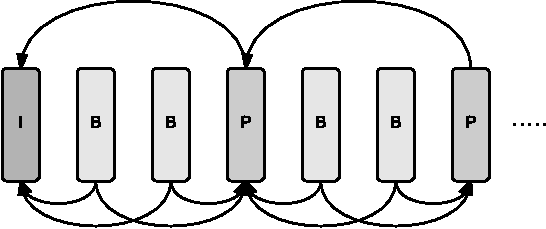
\includegraphics[width=0.7\textwidth]{ipb_chart.pdf}
    \end{center}
    \caption{Схематическое изображение структуры сжатого потока
    для кодека x264 по умолчанию}
    \label{fig:ipb_frames}
\end{figure}

Значительная часть моделей видеотрафика~\cite{} разделяют
сжатый поток кадров разного типа на подпотоки и моделируют
их независимо, получая результирующий поток путём последующего
совмещения подпотоков в соответствии с требуемой схемой.
При таком подходе основной задачей моделирования является
моделирование подпотока одного типа.

В данной работе рассматривается задача моделирования потока
P-кадров, в котором каждый последующий кадр ссылается на
предыдущий. Схема данного потока проиллюстрирована на Рис.~\ref{fig:ippp_frames}.

\begin{figure}[h]
    \begin{center}
        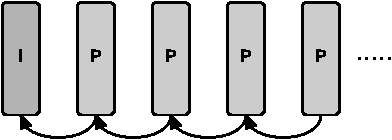
\includegraphics[width=0.55\textwidth]{ippp_chart.pdf}
    \end{center}
    \caption{Схематическое изображение моделируемой структуры сжатого потока
    для кодека x264}
    \label{fig:ippp_frames}
\end{figure}

Таким образом, в задачи данного дипломного проекта входит:

\begin{itemize}
    \item анализ особенностей сжатого VBR-трафика видеоконференций;
    \item обзор существующих моделей VBR-видеотрафика и анализ
        целесообразности их использования при моделировании
        трафика видеоконференций;
    \item реализация набора существующих моделей VBR-видеотрафика
        и методики их адаптации к особенностям трафика видеоконференций;
    \item обзор методов сравнительного анализа моделей;
    \item сравнительный анализ результатов моделирования VBR-трафика
        видеоконференций.
\end{itemize}


\subsection{Анализ особенностей трафика видеоконференций}
\subsubsection{Классификация несжатого видео}
\hspace{3pt}

С точки зрения специалистов в области сжатия видео~\cite{},
видеоданные могут быть условно разделены на классы по
следующим параметрам:

\begin{itemize}
    \item ``активность'' (количество движения) в кадре. Численно 
        эту характеристику можно оценить путём получения разности
        двух последовательных кадров;
    \item ``локальность'' движения. Сосредоточенность энергии
        разностного кадра в конкретных областях кадра;
    \item наличие ``смены сцен''. Смена сцены --- это эвристически
        определяемая резкая перемена освещения, смена плана,
        и тому подобное. Обычно определяется~\cite{} как превышение
        энергии разностного кадра некоторого порога;
    \item геометрические размеры кадра (разрешение)
    \item зашумлённость
    \item требования к качеству сжатого видео: глубина цвета,
        разрешение, соотношение сигнал-шум (PSNR)~\cite{}.
\end{itemize}

Обычно видео разделяют на поддипы по происхождению,
каждый из которых обладает собственным набором признаков.
Для видеопоследовательностей разных классов требуются
различные конфигурации видеокодека или даже разработка
собственного приспособленного под данный класс видеокодека.

\begin{table}{ht}
    \centering
    \begin{tabular}{| c | c | c | c | c | c |}
        & Спорт & CCTV & Conference & Кино & Casual \\
    \end{tabular}
\end{table}
ТАБЛИЦА. Спорт, CCTV, Видеоконференции, Фильмы, Любительская
казуальная видеосъёмка.

В данной дипломной работе объектом моделирования является
сжатый трафик видеоконференций, который в несжатом виде
характеризуется следующими признаками (Таблица~\ref{tab:videotypes}):

\begin{itemize}
    \item малая активность в кадре;
    \item локальный характер движения;
    \item отсутствие смены сцен;
    \item умеренная зашумлённость.
\end{itemize}



\subsubsection{Особенности сжатого видео}
\hspace{3pt}

зависимость автокорреляционной функции от разрешения
и от параметра квантования.

\subsection{Использованное при моделировании тестовое множество}

\subsection{Описание существующих подходов к моделированию VBR-видеотрафика}

\subsection{Критерии сравнительного анализа моделей}
